\section{Design and Implementation}
\label{sec-design}
Our goal is to build a file system for a tiered storage hierarchy consisting of disks and NVM that combines the low latency of NVM with the low cost of disk-based storage, without regressing on performance while offering similar consistency guarantees as BPFS. This seems like a reasonable goal, however, it raises a few non-trivial questions about the overall design of such a tiered filesystem:

\begin{itemize}
\item How do we make changes to BPFS data structures so that it is able to locate the data in the correct tier, i.e. in-memory or disk? \vspace{-0.1in}
\item What policies determine when to move data across the tier? \vspace{-0.1in}
\item Do we handle the disk directly or do we go through another filesystem to store data on the disk? \vspace{-0.1in}
\item What is the ideal granularity at which we should move the data? \vspace{-0.1in}
\end{itemize}

We provide answers to these questions in this section and discuss at length, the policies and mechanisms required to implement the same. Figure~\ref{fig-bpfs} depicts the overall design of our system. We use NVM to store the filesystem metadata and all the filesystem operations are always done within the NVM tier. To preserve the filesystem consistency guarantees, we have opted for a simple design policy where only the data blocks are moved to the disks, while the metadata blocks always reside in the persistent NVM. Such a policy entails that for a given BPFS file, its data may be split across NVM and the disk. However, it is to be noted that even though a data block may be moved between NVM and the disk, there is always a single valid copy of that data block- whether in the disk or in NVM.

The mechanism to determine the exact location of the valid copy of a given data block is implemented using the most significant bit(MSB) of the indirect pointer, pointing to the data block in the BPFS tree structure. If the MSB is not set, then the rest of the 63-bits denote a memory address of the data block within the NVM itself, and if the MSB is set, the rest of the 63-bits denote a disk address where the data block was moved to on the disk. This answers the first question that we had raised earlier. In the following subsections, we discuss the design and implementation of Anti-Cache Manager and the Disk Manager that provide answers to the other design questions.

\begin{figure}
\centering
\vspace{-0.2in}
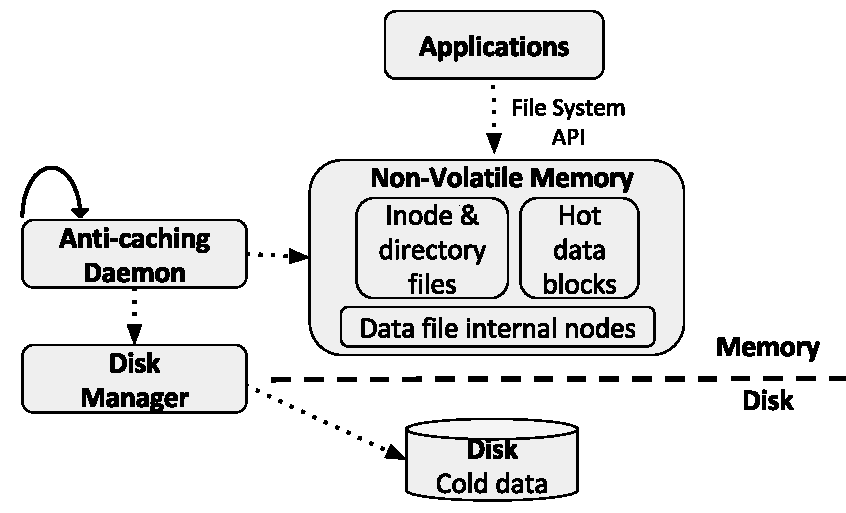
\includegraphics[width=0.5\textwidth]{figs/bpfs.pdf}
\vspace{-0.2in}
\mycaption{fig-bpfs}{Design Architecture of AC-BPFS}{\footnotesize The figure shows the overall design of our system.}
\end{figure}


\subsection{Anti-Cache Manager}
In our design, NVM is the primary data store where all filesystem operations are performed and hence, it contains more frequently accessed blocks. We refer to such data residing in NVM as the `hot' data. Since the capacity of the persistent NVM is limited, we have to periodically evict blocks from NVM to disk, so as to can make space for more `hot' data. The evicted data on the disk is referred to as the `cold' data. While it is true that some of the `hot' data may become `cold' over time, it is also possible that some `cold' data can suddenly become `hot' and it has to be brought back in NVM. This is what we term as the `anti-caching' phenomenon- this gameplay between the `hot' and the `cold' data having a reverse caching effect. This anti-caching is at the heart of our implementation that enables us to amortize the cost of read-write operations equivalent to those provided by BPFS. We implement the well-known LRU-1 policy to distinguish the `hot' data blocks from the `cold' data blocks. We maintain a linked list of all the data block references. Whenever a data block is accessed, it is moved to the front of the linked list. Over time, the tail of the list will contain block references which have been least frequently accessed, while the head of the list will point to data blocks being most frequently accessed.

The anti-cache manager component of the AC-BPFS filesystem implements the above proposed design policies. It runs as a separate background thread that continuously receives a stream of NVM data block references from the main AC-BPFS thread, in the order they are accessed. It maintains an LRU data structure within itself and uses the LRU to evict a number of blocks according to the policy explained above. A soft threshold count of data blocks, known as `anti-caching threshold', is used to determine when and how many blocks to evict. The anti-cache manager is made to poll arbitrarily every 10 ms on the size of the LRU list. If the size of the LRU list exceeds the specified anti-caching threshold of data blocks count in NVM, those many extra data blocks over the threshold are evicted from the tail of the list. This anti-caching threshold is set based on the latency of NVM writes and the polling time. We found that setting the anti-caching threshold to 80\% of the NVM size for a 10 ms polling duration is a good estimate. In order to ensure that data blocks that are currently being evicted to disk do not get updated by the file  system, a block level locking mechanism is used which implicitly prevents any updates to the block.

This subsection answered our second question on the policies required to move data between NVM and the disk. The next subsection gives the answers to the remaining two questions.

\subsection{Disk Manager}
The disk manager component of AC-BPFS is responsible for managing the data blocks on the disk. It stores the evicted cold blocks from NVM, as well as, provides the data blocks back to the main AC-BPFS thread when requested. As explained earlier, our policy is to move only the data blocks between the disk and NVM. We have opted for a fixed 4 KB granularity as the size of a disk block, which is the same size of a BPFS in-memory data block. Thus, each data block on the disk is aligned at a 4 KB disk address. We found that it to be simpler to use a well-known filesystem like ext4 for our disk-based filesystem operations than to create our own filesystem. Hence, the disk manager simulates a virtual disk using a single file stored on disk in the ext4-mounted partition of a predetermined size. It exposes the usual filesystem APIs for reading and writing blocks into the disk. As and when the blocks are evicted by the anti-cache manager, they are written to the disk. When the blocks are moved back into the NVM, they leave holes in the file which can cause the file to become fragmented. To solve this fragmentation problem, we keep a free list of the holes that point to disk addresses of the blocks that have been moved to NVM and now can be reused.

The disk manager also buffers a set of writes in the DRAM buffer cache to optimize the \textit{write} latency by writing the blocks in bulk. Our current implementation provides consistency at the expense of performance by notifying BPFS only after persisting the blocks. The indirect pointers in the inodes are updated atomically to point to the disk addresses of the evicted blocks through a synchronous call. To speed up the loading of blocks back into NVM from the disk, we perform prefetching of additional blocks into DRAM when a read is performed. The lifetime of the prefetched blocks in memory is predetermined to ensure that unused prefetched blocks are cleaned up regularly.

\subsection{File System Operations}
In this section we describe the workflows for various file system operations.
\subsubsection{Read}
When a read operation is performed on a file, the main AC-BPFS thread crawls the inode tree to determine the indirect block containing the pointer to the data block. Then, it identifies the location of the data block using the MSB that indicates whether the block is on the disk or in NVM. If the block is on the disk, then it fetches the block into NVM. Once the block is persisted in NVM, it frees the block on the disk and updates the indirect pointer in the inode tree to point to the new block location in NVM atomically.

\subsubsection{Write}
When a \textit{write} operation is performed on a file, the main AC-BPFS thread traverses the inode tree to find the indirect block containing the pointers to the data block of the file and identifies the location of the data blocks. If the data block is in NVM, the \textit{write} operation is performed in-place and has no additional overhead. If the data block is on disk, the block is fetched into NVM thus performing a copy-on write of the data block and this block is updated and written back to NVM. The block on disk is then freed and the control comes back to the crawler. The indirect pointer in the inode tree is then updated to point to this new block location in-place along with in-place writes of the other internal nodes. The inode access time is also updated through an in-place atomic write.

\subsubsection{Open}
When a file is opened, the directory inode tree is parsed to find the file. If the file is not found and a create is requested, a new inode number is generated and the new inode is written to the inode file. Then the directory file is updated. All these updates are performed in-place. Since the metadata updates are in-place and in NVM, they are faster than usual disk writes and the additional overhead of metadata journaling can also be saved by avoiding disk writes.
